\documentclass[aspectratio=169]{beamer}


%%% PAQUETES  %%%
%%% PAQUETES  %%%


%%% TODONOTES y definición 2cm de margen para que no se solapen añadido colores comentarios
\setlength {\marginparwidth }{2cm} 
\usepackage{todonotes}
\usepackage[normalem]{ulem}

\usepackage[normalem]{ulem}

%%%%%%%%%%%%%%%%%%%%%%%%%%%%%%%%%%%%%%%%%%%%%%%%%%%%%%%%%%%%%%%%%%%%%%%%%%%%%%%%%

%%% Tildes y demás caracteres en español...
%\usepackage[latin1]{inputenc}
% o bien
\usepackage[utf8]{inputenc}

%%% Fuente Times...
\usepackage{times}

%%% Figuras en formato .png, .ps, pdf o eps
\usepackage{graphicx}
\usepackage{subfigure}
\DeclareGraphicsExtensions{.png,.eps,.ps,.pdf}

%%% Soporte graficos svg
\usepackage{svg}

%%% Formato y tipografía de URL, direcciones de correo...
\usepackage{url}
%\usepackage{hyperref}

%%% Sección para definir explícitamente la separación de sílabas al final de una línea:
\hyphenation{si-guien-do}

%%% Secciones etc. en castellano
\usepackage[spanish,es-tabla]{babel}

%%% Paquete para poner hipervinculos más finos \href
\usepackage{hyperref}

\hypersetup{
    colorlinks=true,
    linkcolor=black,
    filecolor=black,
    %%% Necesita su propia definicion de color
    citecolor=dimgray,  
    urlcolor=coolblack,
}



\usepackage{xcolor}

%%% Paquete para comentarios
\usepackage{verbatim}

% Definiciones colores extra
%% Ref: http://latexcolor.com/
	\definecolor{coolblack}{rgb}{0.0, 0.18, 0.39}
	\definecolor{dimgray}{rgb}{0.41, 0.41, 0.41}


%%% Paquete para usar simbolos y scripts de dibujado
\usepackage{tikz}
\def\checkmark{\tikz\fill[scale=0.4](0,.35) -- (.25,0) -- (1,.7) -- (.25,.15) -- cycle;} 
\usetikzlibrary{shapes,arrows}

% Define Block styles
\tikzstyle{decisionBL} = [diamond, draw, fill=blue!20,text width=10em, text badly centered, node distance=3cm, inner sep=0pt]
\tikzstyle{blockBL} = [rectangle, draw, fill=blue!20,text width=9em, text centered, rounded corners, minimum height=4em]
\tikzstyle{blockYL} = [rectangle, draw, fill=yellow!20, text width=9em, text centered, rounded corners, minimum height=4em]
\tikzstyle{blockGR} = [rectangle, draw, fill=green!20, text width=9em, text centered, rounded corners, minimum height=4em]
\tikzstyle{blockRD} = [rectangle, draw, fill=red!20, text width=9em, text centered, rounded corners, minimum height=4em]
\tikzstyle{blockWH} = [rectangle, draw, fill=white!20, text width=9em, text centered, rounded corners, minimum height=4em]
\tikzstyle{line} = [draw, -latex']
\tikzstyle{cloud} = [draw, ellipse,fill=red!20, node distance=4.5cm,minimum height=4em]

%%% Para usar ficheros tex de infografias Inkscape
\usepackage{pstricks}
%\definecolor{Azuloscuro-cisis}{RGB}{1,62,133}
\definecolor{Azulclaro-cisis}{RGB}{0,101,219}

\definecolor{LUCopper}{rgb}{0.8,0,0} %títulos slides
\definecolor{LUBlue}{rgb}{0.07, 0.04, 0.56}

\definecolor{LUPink}{rgb}{0.24,0.82,0.44}
\definecolor{LUGreen}{rgb}{0.24,0.82,0.44}
\definecolor{LUWhite}{rgb}{1,1,1} % fondo
%%% COMANDOS  %%%
%%% COMANDOS  %%%

%%% A cursiva  %%%
\newcommand{\cursiva}[1]{\em{#1}}


%%% Fuzzing en bonito  %%%
\newcommand{\fz}{\em fuzzing}

%%% Atajos estilo  %%%

\newcommand{\CLASSINPUTinnersidemargin}{18mm}
\newcommand{\CLASSINPUToutersidemargin}{12mm}
\newcommand{\CLASSINPUTtoptextmargin}{20mm}
\newcommand{\CLASSINPUTbottomtextmargin}{25mm}

\newcommand{\new}[1]{\textcolor{olive}{{#1}}}
%\newcommand{\old}[1]{\textcolor{purple}{{\sout{#1}}}}
\newcommand{\wip}[1]{\textcolor{blue}{{#1}}}
%\newcommand{\checkthis}[1]{\textcolor{orange}{{#1}}}
\newcommand{\diego}[1]{\textcolor{magenta}{{#1}}}
\newcommand{\vmodixit}[1]{\textcolor{teal}{{#1}}}

\newcommand{\old}[1]{\textcolor{purple}{{\sout{#1}}}}
\newcommand{\camino}[1]{\textcolor{olive}{{#1}}}
\newcommand{\fjrodl}[1]{\textcolor{blue}{{#1}}}
\newcommand{\checkthis}[1]{\textcolor{orange}{{#1}}}

%%% Entornos  %%%
\newcounter{definicion}
\newenvironment{definicion}[1]{%
    \refstepcounter{definicion}\par\medskip%
    \noindent \textbf{Definición~\thedefinicion. #1}.\ %
}{\medskip}

%%%% Soporte para el logo de ORCID
%\newcommand{\orcid}[1]{\href{https://orcid.org/#1}{\textcolor[HTML]{A6CE39}{\aiOrcid}}}



\title[{\fz} robots HPC \& LLM]{\textbf{Fuzzing Robotic Software using HPC and LLM}\\
%\tiny \\
%\tiny y desacoplada para el uso de técnicas de {\fz} en HPC.\\
\small{\underline{Francisco Borja Garnelo Del Río}, Francisco J. Rodríguez Lera } \\
\small{Camino Fernández Llamas, Vicente Matellán Olivera} \\
\tiny{Universidad de León - 
Campus de Vegazana s/n, 24071 León (Spain)} \\
\tiny{infbgd01@estudiantes.unileon.es, \{fjrodl, cferll, vmato\}@unileon.es}
}

\titlecolor{LUWhite} % Choose between LUPink, LULBlue, LUIvory, LUGreen


% Titulo como imagen conferencia2024.pn
%        Computational Intelligence in Security for Information Systems
%            17th International conference 9-11 October 2024

\titleimage{\includegraphics[scale=0.55]{./img/conferencia2024.png}}

\author{Francisco B. Garnelo del Río (infbgd01@estudiantes.unileon.es)}

%\subtitle{\\ 
%\small{\underline{\\Francisco Borja Garnelo Del Río}, \\Francisco J. Rodríguez Lera,}\\ 
%\small{Camino Fernández Llamas, Vicente Matellán Olivera} \\
%\tiny{Universidad de León - Campus de Vegazana s/n, 24071 León (Spain)} \\
%\tiny{infbgd01@estudiantes.unileon.es, \{fjrodl, cferll, vmato\}@unileon.es}
%} 

\date{CISIS 2024}

\begin{document}
%\renewcommand{\contentsname}{Contenidos}
%\renewcommand{\figurename}{Figura}
%\renewcommand{\tablename}{Tabla}
%\renewcommand{\sectionname}{Sección}
%\renewcommand{\subsectionname}{Subsección}
%\renewcommand{\partname}{Parte}

%% TODO: Actualizar tabla una vez cerrada estructura.

\titleframe

\begin{frame}{Table of Contents}

\begin{enumerate}
\item Introduction
\begin{itemize}
    \item Research Objectives
    \item State of the art
\end{itemize}
\item Materials and Methods
\begin{itemize}
    \item Infrastructures
    \item Software
\end{itemize}
\item Proof-of-Concept Design
\begin{itemize}
    \item Simulation
    \item Integration
    \item Validation    
\end{itemize}    
\item Contribution
\item Conclusions and Future Work
\end{enumerate}
 \end{frame}

 %% REF: Cajas https://texdoc.org/serve/tcolorbox.pdf/0

 % INTRODUCCION %%%%%%%%%%%%%%%%%%%%%%%%%%%%%%%%%%%%%%%%%%%%%%%%%
\begin{comment}  
\section{Introduction}
%\frame{\sectionpage}
\begin{frame}{Introduction}

 
  \only<1>{
    
\begin{tcolorbox}[drop shadow southeast,
enhanced,colback=blue!5!white,colframe=Azuloscuro-cisis]
\textbf{Large Language Model (LLM)}is a type of artificial intelligence designed to understand and generate human-like text based on vast amounts of data. It uses deep learning techniques to predict and produce coherent and contextually relevant language outputs.
\end{tcolorbox}


\begin{tcolorbox}[drop shadow southeast,
enhanced,colback=blue!5!white,colframe=Azuloscuro-cisis]
\textbf{Fuzzing} is the automation of generating and testing malformed inputs in software in order to find unexpected behavior in the software.
\end{tcolorbox}

\begin{tcolorbox}[drop shadow southeast,
enhanced,colback=blue!5!white,colframe=Azuloscuro-cisis]
\textbf{Robotic systems} are systems that interact with their environment, including people, through the use of numerous sensors, actuators, and user interfaces to give intelligent services and information.
\end{tcolorbox}

\begin{tcolorbox}[drop shadow southeast,
enhanced,colback=blue!5!white,colframe=Azuloscuro-cisis]
\textbf{High Performance Computing (HPC)} is a technique that processes huge multidimensional information and solves complex problems at incredibly fast rates by using clusters of powerful processors operating in parallel.
\end{tcolorbox}
}
\end{frame}
\end{comment}



\section{Introduction}
%\frame{\sectionpage}

%%% Introduction %%%%%%%%%%%%%%%
%% REVISAR: TODO:Problema a solucionar, como ayuda, automatizando pruebas en SW, ahora en robots, y en esta ultima linea generando inputs con IA con lenguaje natural. (Vender la historia como se hace, el frame, librerias, robot, tools, carga de trabajo...)
\begin{frame}{Introduction}

\only<1>{

\begin{tcolorbox}[drop shadow southeast,
enhanced,colback=blue!5!white,colframe=Azuloscuro-cisis]
\textbf{Challenges in Robotic Software Testing:}
\begin{itemize}
    \item Traditional software testing methods are insufficient for complex robotic systems.
    \item Need for extensive computational resources for fuzz testing.
\end{itemize}
\end{tcolorbox}

\begin{tcolorbox}[drop shadow southeast,
enhanced,colback=blue!5!white,colframe=Azuloscuro-cisis]
\textbf{Innovative Approach:}
\begin{itemize}
    \item Development of a modular, scalable testing framework (HOUSE).
    \item Utilizing HPC for scalable and robust testing environments.
    \item AI-driven input generation for fuzz testing based on natural language commands.
\end{itemize}
\end{tcolorbox}

}

\end{frame}

%%% Concepts %%%%%%%%%%%%%%%
\subsection{Concepts}
%\frame{\sectionpage}
\begin{frame}{Introduction - Concepts}
 
  \only<1>{

\begin{tcolorbox}[drop shadow southeast,
enhanced,colback=blue!5!white,colframe=Azuloscuro-cisis]
\textbf{Large Language Model (LLM)} is an AI designed to understand and generate human-like text using deep learning on vast data.
\end{tcolorbox}

\begin{tcolorbox}[drop shadow southeast,
enhanced,colback=blue!5!white,colframe=Azuloscuro-cisis]
\textbf{Fuzzing} automates the generation and testing of malformed inputs to find unexpected software behavior.
\end{tcolorbox}

\begin{tcolorbox}[drop shadow southeast,
enhanced,colback=blue!5!white,colframe=Azuloscuro-cisis]

%% REVISAR: Definicion de ROS2 framwework
%% OLD: \textbf{Robotic systems ROS2} \textbf{TODO}: Cambiar por enfoque a framework de sistema robotico.
\textbf{ROS2 framewoek} Provides a flexible architecture for building and deploying complex robotic systems.

\end{tcolorbox}

\begin{tcolorbox}[drop shadow southeast,
enhanced,colback=blue!5!white,colframe=Azuloscuro-cisis]
\textbf{High Performance Computing (HPC)} uses clusters of powerful processors to solve complex problems quickly.
\end{tcolorbox}


}

\end{frame}

%%% Framework and Tools Overview %%%%%%%%%%%%%%%
\subsection{Framework and Tools Overview}
\begin{frame}{Introduction - Framework and Tools Overview}

\only<1>{

\begin{tcolorbox}[drop shadow southeast,
enhanced,colback=blue!5!white,colframe=Azuloscuro-cisis]
\textbf{House framework Components:}
\begin{itemize}
    \item \textbf{HPC Support:} Enables large-scale testing.
    \item \textbf{Fuzzing Techniques:} Automated input generation and mutation.
    \item \textbf{AI Integration:} Natural language processing for intelligent input generation.
\end{itemize}
\end{tcolorbox}

\begin{tcolorbox}[drop shadow southeast,
enhanced,colback=blue!5!white,colframe=Azuloscuro-cisis]
\textbf{Key Tools:}
\begin{itemize}
    \item \textbf{RoboFuzz:} Core robotic fuzzing tool.
    \item \textbf{Marcoroni LLM:} AI model for generating test inputs.
    \item \textbf{Singularity:} Container technology for deployment.
\end{itemize}
\end{tcolorbox}

}

\end{frame}



%%% Research Objectives %%%%%%%%%%%%%%%
\subsection{Research Objectives}
%\frame{\subsectionpage}
\begin{frame}{Introduction - Research Objectives}
  \only<1>{

%\begin{tcolorbox}[drop shadow southeast,
%enhanced,colback=blue!5!white,colframe=Azuloscuro-cisis,title=Research question ]
%What are the implications of using HPC systems when fuzzing ROS applications?
%\end{tcolorbox}

Main research Objectives:

\begin{tcolorbox}[drop shadow southeast,
enhanced,colback=blue!5!white,colframe=Azuloscuro-cisis]

\begin{itemize}
    \item \textbf{Enhance Cybersecurity} Apply fuzzing to improve the security of complex robotic software using an open-source tool with publicly available code, integrated into a system that supports horizontal scaling. 
    \item \textbf{Utilize LLM} Integrate generative AI methodologies in the fuzzing process, particularly in message generation and mutation.
    \item \textbf{Leverage HPC} Implement and evaluate the use of HPC, building on previous work, to support horizontal scaling compatible with HPC environments.    
\end{itemize}

\end{tcolorbox}
}


\end{frame}






\begin{comment}
    
%%% Goals and Hypotheses %%%%%%%%%%%%%%%
\subsection{Goals and Hypotheses}
%\frame{\subsectionpage}
\begin{frame}{Introduction - Goals and Hypotheses}
  \only<1>{

\begin{tcolorbox}[drop shadow southeast,
enhanced,colback=blue!5!white,colframe=Azuloscuro-cisis,title=Research question ]
What are the implications of using HPC systems when fuzzing ROS applications?
\end{tcolorbox}

This question arises from the following hypothesis and questions: 

\begin{tcolorbox}[drop shadow southeast,
enhanced,colback=blue!5!white,colframe=Azuloscuro-cisis]

\begin{itemize}
    \item \textbf{H1:} Distributing the fuzzing workload across multiple processing units can significantly increase overall fuzzer performance. 
    \item \textbf{Q1:} What are the key concepts associated with Fuzzing in HPC?
    \item \textbf{Q2:} What is the performance of the fuzzer when running in a personal computer or HPC computer?    
\end{itemize}

\end{tcolorbox}
}



\end{frame}
\end{comment}


\begin{comment}
    

%%% State of the art %%%%%%%%%%%%%%%
 \subsection{State of the art}
%\frame{\subsectionpage}
\begin{frame}{Introduction - State of the art}

  \only<1>{

\begin{itemize}
    \item \textbf{Fuzz Testing Origins:} Fuzz testing, or fuzzing, originated from a UNIX security study in the 1990s and has been crucial in uncovering software vulnerabilities and programming errors.
    \item \textbf{Advancements in Fuzzing:} Recent advancements include grammar-based fuzzing, symbolic execution, taint-based fuzzing, and neural network-based fuzzing to improve input generation and code coverage.
    \item \textbf{Fuzzing in ROS2:} Active research focuses on enhancing the robustness and security of ROS2 robotic systems, identifying vulnerabilities through unexpected and invalid inputs.
   % \item \textbf{RoboFuzz Framework:} Development of RoboFuzz automates fuzz testing for ROS2 systems.

\end{itemize}
 }

\end{frame}
\end{comment}

 
 \section{Materials and Methods}
%\frame{\sectionpage}
%\begin{frame}{Materials and Methods}
%This section will present everything %related to:
%\begin{itemize}
%    \item Infrastructures
%    \item Software
%    \item Experiments
%    \item Implemented cases
%\end{itemize}
%\end{frame}

 \subsection{Infrastructures}
%\frame{\subsectionpage}
\begin{frame}{Materials and Methods - Infrastructures}
Each experiment was tested on two different infrastructures:
\begin{itemize}
    \item \textbf{Standalone} SDO,  virtual machine with 8GB ram and 6 x Intel Xeon E3-12xx v2 vcpu (virtual cpu) and linux kernel \textit{5.3.11-100.x86\_64 (x86\_64)}. Local storage on mechanical hard disks.
  
    \item \textbf{High-Performance Computing} HPC, computing cluster with Haswell nodes in bare-metal with 48GB of ram and 2 x Intel Xeon E5-2630 v3 @ 3.20GHz with a total of 16 cores and a Linux kernel \textit{3.10.0-1062.9.1.x86\_64 (x86\_64) } .
      Network storage and cache on solid disks. %The HPC manager has been used to manage the distribution of the executions, you can see in the .slurm files used the details, mainly the common HPC policy has been used to share cpu and ram resources, allowing up to 32 parallel tasks per node. 
      
\end{itemize}
\textit{NOTE: When using containers the distro is indifferent.}
\end{frame}
 
 \subsection{Software}
%\frame{\subsectionpage}
\begin{frame}{Materials and Methods - Software}
The experiments made use of the following software:

\begin{itemize}
    \item \textbf{RoboFuzz}, an autonomous fuzz testing tool for robotic systems. 
    \item \textbf{SLURM} (Simple Linux Utility for Resource Management) a widely used open-source workload manager and job scheduler for Linux and Unix-based clusters and supercomputers.
    \item \textbf{Singularity} a container solution created to run complex applications on HPC clusters in a simple, portable, and reproducible way.
    \item \textbf{Docker}, an open container platform for developing, shipping, and running applications.
    \item \textbf{Marcoroni 7B V3-GGUF}, an auto-regressive language model designed for the English language, integrated into ROS2 using the llama\_ros package  .    
\end{itemize}

\end{frame}

%%% TODO: No logro separar esta subseccion en 3 diapositivas  
\section{Proof-of-Concept Design}

\begin{frame}{Proof-of-Concept Design - TODO:Fuzzing }
 \textbf{TODO:} Meter lo de ciclo de fuzzing (ver captura telegram). Ligarlo con tema de empresa y academia para temas de validación.

\end{frame}

%%% TODO: No logro separar esta subseccion en 3 diapositivas  
\section{Proof-of-Concept Design}
\subsection{Simulation}
\begin{frame}{Proof-of-Concept Design - Simulation}
 \textbf{Simulation with Turtlebot3(tb3) robot:} Conducted fuzzing on a differential wheeled mobile robot equipped with a LiDAR sensor designated topics.

\textbf{TODO: } Meter imagen de un turtlebot para que lo vean, y aclarar que es un robot para pruebas y experimentación. Explicar la estrategia que es por robot y topic.

\end{frame}

\section{Proof-of-Concept Design}
\subsection{Simulation}
\begin{frame}{Proof-of-Concept Design - Simulation}
 \textbf{Simulation with Turtlebot3(tb3) robot:} Conducted fuzzing on a differential wheeled mobile robot equipped with a LiDAR sensor designated topics.

\textbf{TODO: } Meter imagen de un turtlebot para que lo vean, y aclarar que es un robot para pruebas y experimentación. Explicar la estrategia que es por robot y topic.
%\begin{figure}[htbp]
\begin{figure}[ht!]
    \centering
    \includesvg[width=1.0\textwidth]{./figures/data/rqt_graph/all/llama_ros-tb3.svg}
    %\caption{rqt\_graph associated all active nodes and topics during the validation process.}
    \label{fig:robofuzz_rqt_graph_all_llama_ros-tb3}
\end{figure}

\end{frame}

    
\subsection{Integration IA}
\begin{frame}{Proof-of-Concept Design - Integration IA}
 \textbf{Integration of GenAI:} Expanded RoboFuzz's input management capabilities to utilize LLM or VLM models compatible with llama.cpp  .
 %%\begin{figure*}[p!]
%\begin{figure*}[ht!]
\begin{figure}[ht!]
%%https://www.overleaf.com/learn/latex/Positioning_of_Figures
    \centerline{
    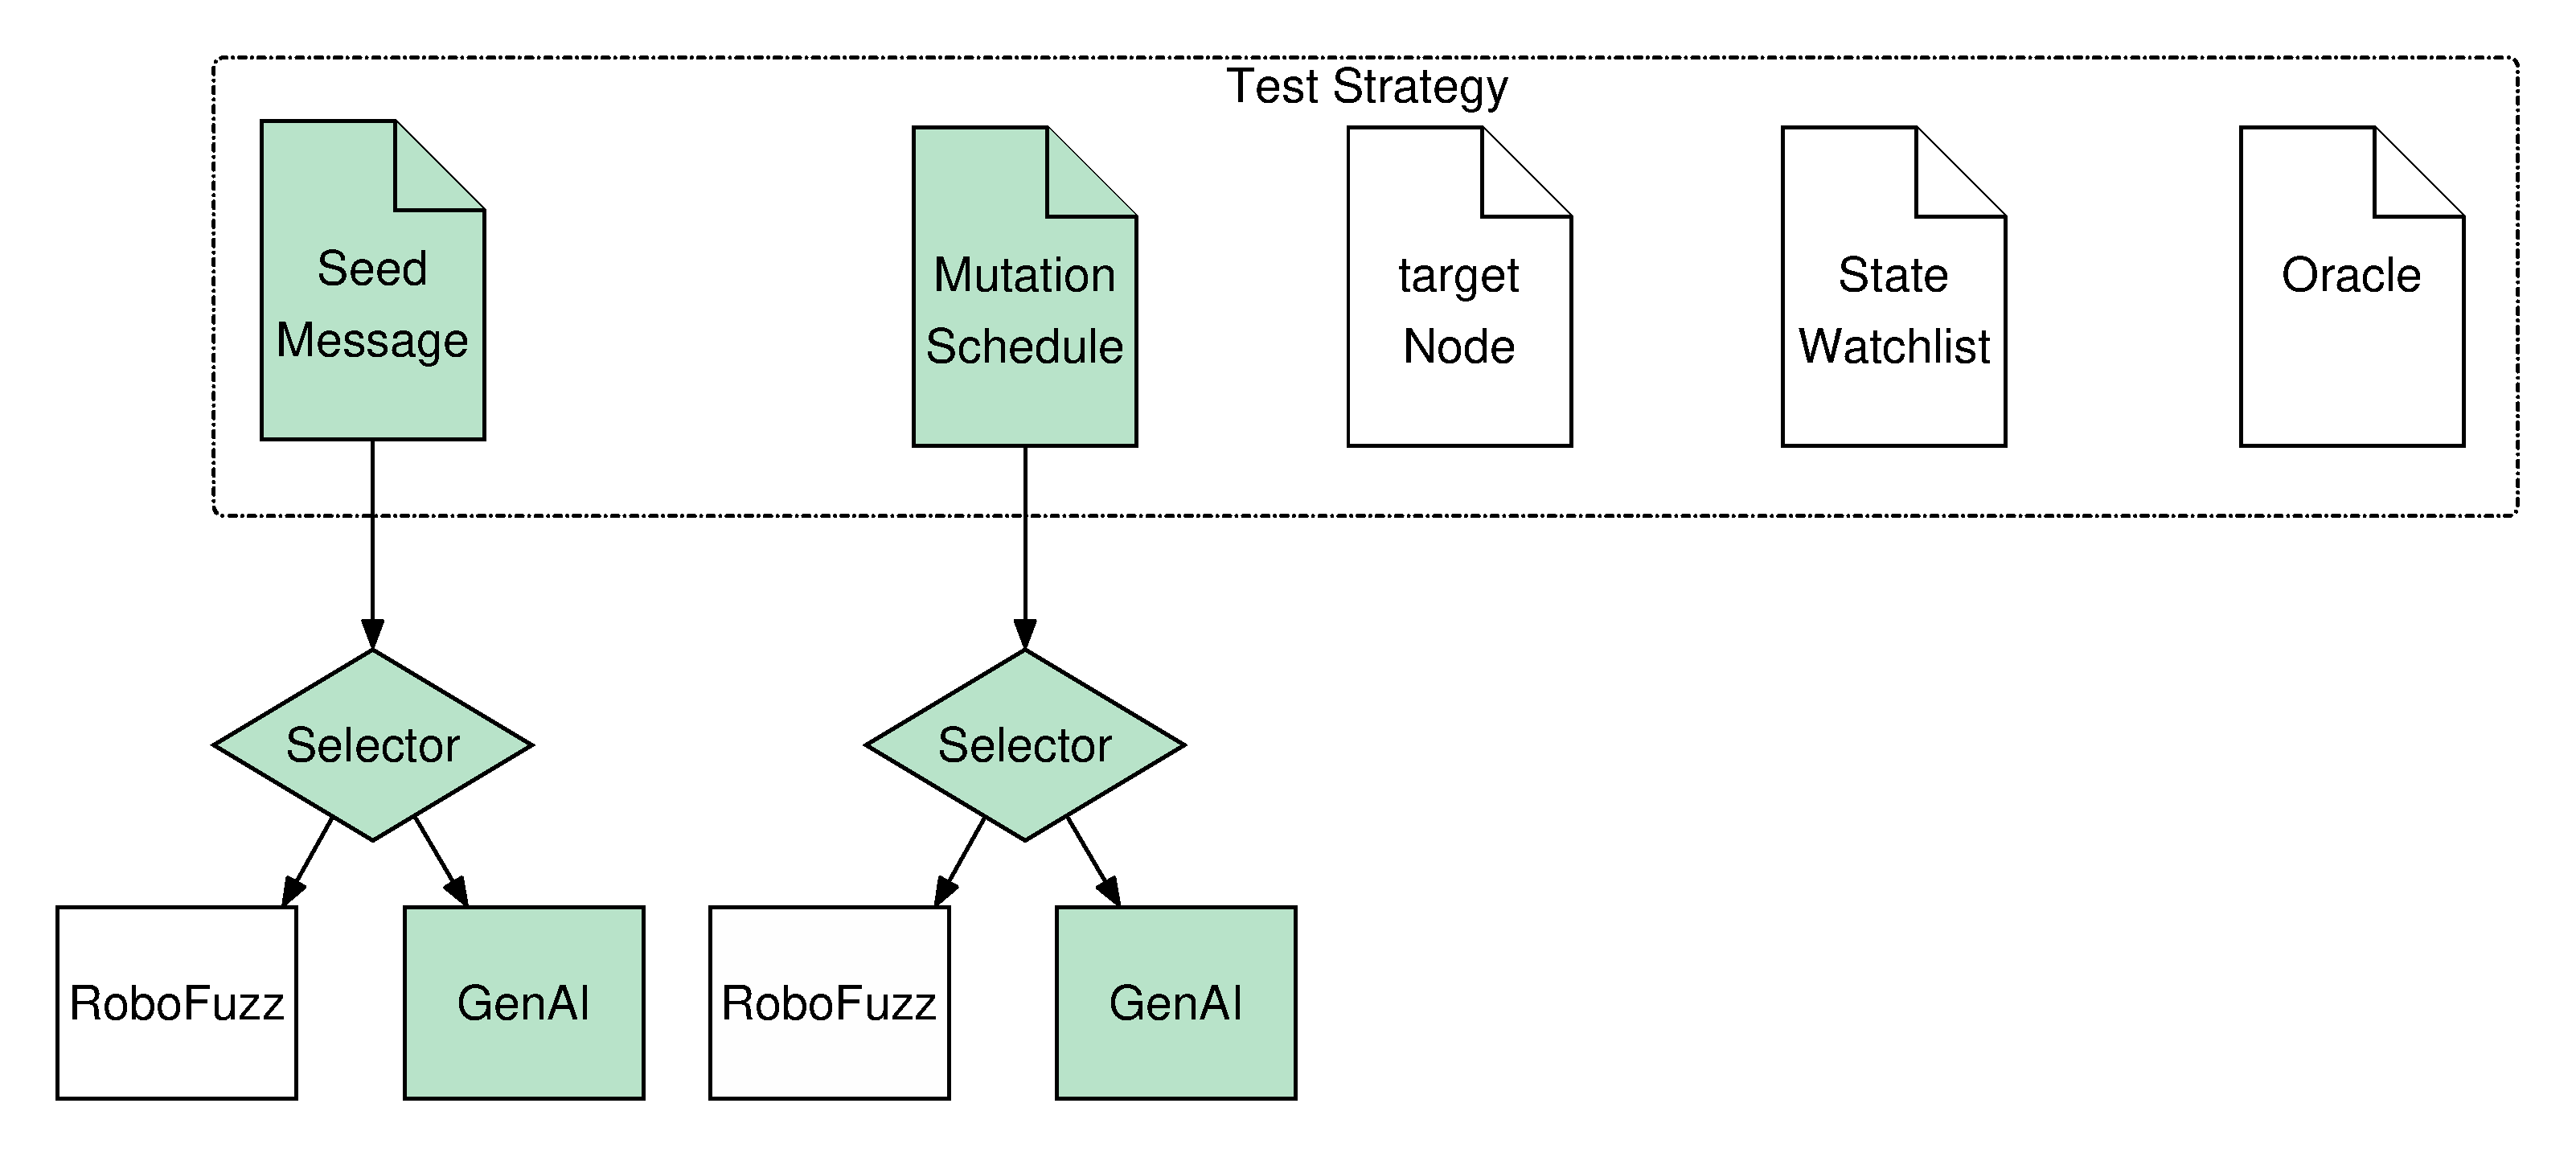
\includegraphics[width=0.7\linewidth]{ ./figures/data/Test_Strategy.pdf}}
    \caption{The input test strategies of RobotFuzz, inclusive of the genai module features.}
    \label{fig:genai-robofuzz_test_strategy}
\end{figure} 
\end{frame}

\subsection{Validation}
\begin{frame}{Proof-of-Concept Design - Validation}
 \textbf{Validation Process:} Detailed logs and statistics of the fuzzing process, including seed generation and mutation.
%%\begin{figure}[htbp]
\begin{figure}[ht!]
    \centering
    \includegraphics[width=1\textwidth]{./figures/data/robofuzz_genai_02_fase2_mutaciones.png}
    \caption{The operation of the GenAI module in mutation.}
    \label{fig:robofuzz_genai_02_fase2_mutaciones}
\end{figure} 
%\begin{figure}[htbp]
\begin{figure}[ht!]
    \centering
    \includegraphics[width=1\textwidth]{./figures/data/robofuzz_genai_00_fase1-fase2.png}
    \caption{The operation of the GenAI module in seed generation and mutation.
.}
    \label{fig:robofuzz_genai_00_fase1-fase2}
\end{figure}
\end{frame}

\subsection{Validation}
\begin{frame}{Proof-of-Concept Design - Validation}
 \textbf{TODO:} Resaltar lo que son logs solo para explicarlos.
%%\begin{figure}[htbp]
\begin{figure}[ht!]
    \centering
    \includegraphics[width=1\textwidth]{./figures/data/robofuzz_genai_02_fase2_mutaciones.png}
    \caption{The operation of the GenAI module in mutation.}
    \label{fig:robofuzz_genai_02_fase2_mutaciones}
\end{figure} 
%%\begin{figure}[htbp]
\begin{figure}[ht!]
    \centering
    \includegraphics[width=1\textwidth]{./figures/data/robofuzz_genai_00_fase1-fase2.png}
    \caption{The operation of the GenAI module in seed generation and mutation.
.}
    \label{fig:robofuzz_genai_00_fase1-fase2}
\end{figure}
\end{frame}


\section{Contribution}
\begin{frame}{Contribution}
\begin{tcolorbox}[drop shadow southeast, enhanced, colback=blue!5!white, colframe=Azuloscuro-cisis]
\begin{itemize}
    \item \textbf{Integration of LLM:} Developed a new module, GenAI, for RoboFuzz to utilize Large Language Models (LLM) in the seed generation and mutation process.
    \item \textbf{AI-Driven Fuzzing:} Replaced the traditional Mutator module with a generative AI model, enhancing the efficiency and effectiveness of fuzz testing.
    \item \textbf{Modular Design:} Designed for modular utilization with Singularity container technology, facilitating large-scale deployment in High-Performance Computing (HPC) environments.
    \item \textbf{Open Source Tool:} Provided a ready-to-use deployable tool with all associated materials, including the proof of concept and code, accessible on GitHub for review and utilization.
\end{itemize}
\end{tcolorbox}
\end{frame}

% Slide for Conclusions and Future Work
\section{Conclusions and Future Work}
\begin{frame}{Conclusions and Future Work}
\begin{tcolorbox}[drop shadow southeast, enhanced, colback=blue!5!white, colframe=Azuloscuro-cisis]
\begin{itemize}
    \item \textbf{Conclusions:}
    \begin{itemize}
        \item Demonstrated the viability and potential of integrating generative AI within an HPC environment for fuzz testing.
        \item Highlighted the benefits of using AI for automated input generation and mutation, improving the robustness and security of ROS2-based robotic systems.
    \end{itemize}
    \item \textbf{Future Work:}
    \begin{itemize}
        \item Explore the use of more specific AI models tailored for different tasks to enhance the quality of fuzz testing.
        \item Investigate the performance of AI-optimized hardware to improve the efficiency of generative AI models.
        \item Expand the application of the developed framework to other domains and robotic systems.
    \end{itemize}
\end{itemize}
\end{tcolorbox}
\end{frame}

% PREGUNTAS %%%%%%%%%%%%%%%%%%%%%%%%%%%%%%%%%%%%%

\begin{frame}
%\begin{frame}[plain,standout]
\begin{center}
\vspace*{\stretch{1}}
{\centering\Huge\textcolor{black!50}{Thank you for your attention.}\par Do you have any questions?}%
\vspace*{\stretch{1}}
\end{center}
    
\end{frame}

%\titleframe
%\appendix

% REFERENCIAS %%%%%%%%%%%%%%%%%%%%%%%%%%%%%%%%%%%%%
%
%\begin{frame}[allowframebreaks]{References}
%
%    \bibliographystyle{spmpsci}
%    \bibliography{bibliography.bib}
%
%\end{frame}


\end{document}

